\documentclass[12pt]{article}   % stay with the familiar article class
\usepackage{reportstyle}        % <— all customisations arrive here
\usepackage{subcaption}
% Make subfigure references appear as 2(a), 2(b)
\captionsetup[subfigure]{labelformat=simple}
\renewcommand\thesubfigure{(\alph{subfigure})}
\DeclareSIUnit{\decade}{dec}

% helper: define only if still undefined
\providecommand{\moduleheader}[1]{}
\providecommand{\titleimage}[1]{}
\providecommand{\titleimageheight}[1]{}

% --- front-matter settings specific to *this* report ---
\title{Analogue Electronics (Project) 4 Simulation Project Report}
\author{Steven \\ s2291752}
\date{\today}
\moduleheader{Analogue Electronics (Project) 4}

% optional image settings
\titleimage{Analogue\_electronics}          % file must be present
\titleimageheight{0.3\textheight}   % tweak height

\begin{document}
	
	\maketitle
	
	\section{Exercise 1: Transistor parameter extraction}
	
	In this section of exercise, I'm going to simulate the transistors in Cadence Virtuoso, and extract some parameters from the simulation result using a simple transistor model. Finally, I'll analysis some questions based on the extracted parameters and the theoretical model. The first simulation is a plot of a group of $I_d$ against $V_{DS}$ under different value of $V_{GS}$, this is shown in Figure \ref{fig:groupIdVds}.

	\begin{figure}[htbp]
		\centering
		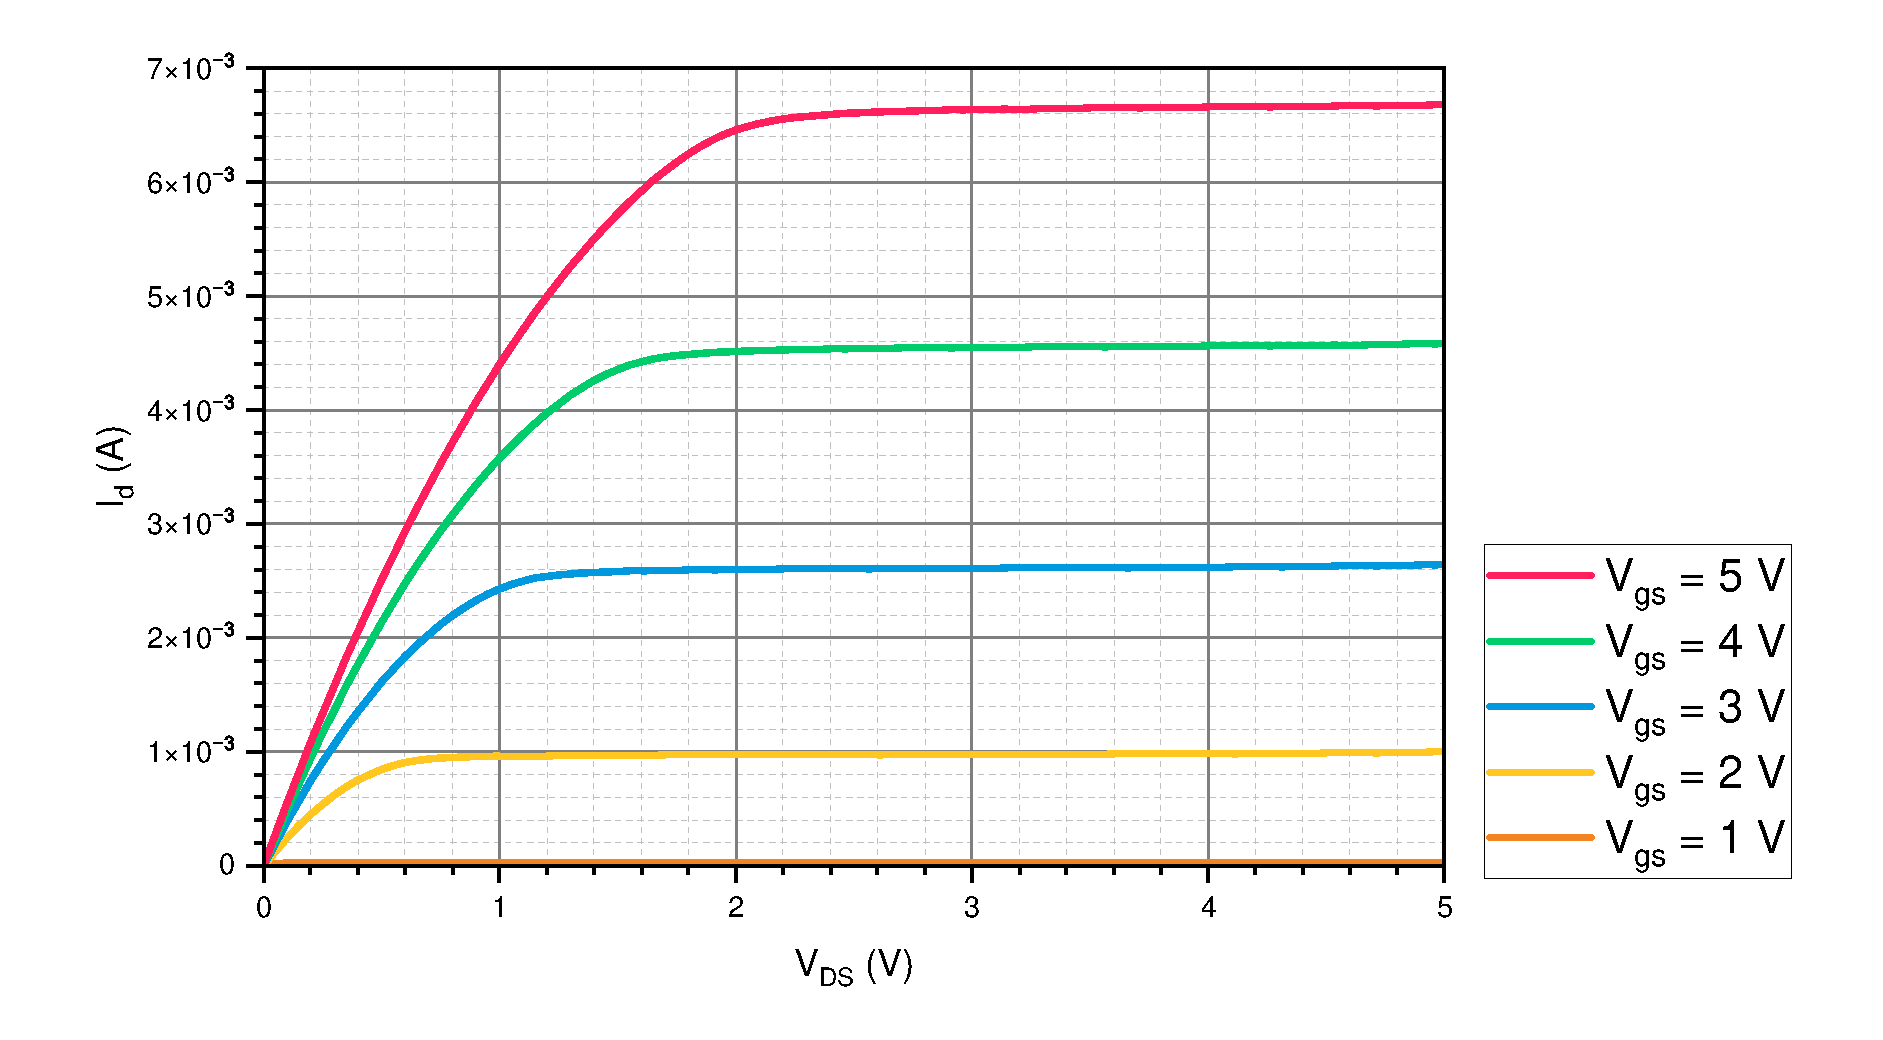
\includegraphics[width=0.7\linewidth]{Figures/E1_NMOS_Characteristic/Group_Id_VDS}
		\caption{The plot of $I_d$ against $V_{DS}$ under 5 different $V_{GS}$}
		\label{fig:groupIdVds}
	\end{figure}
	
	Considering the plot which $V_{GS} = \SI{2}{\volt}$, the curve in the saturation region could be expressed as equation \eqref{eq:idsSat}. The parameter $\lambda$ in the equation is used to model the channel-length modulation effect of the transistor.
	\begin{equation}
		I_{DS} = \beta \left(V_{GS} - V_{T}\right)^2 \left(1 + \lambda V_{DS}\right)
		\label{eq:idsSat}
	\end{equation}
	Substitute two groups of $V_{DS}$ and $I_{DS}$ and take the ratio of them:
	\begin{equation}
		\frac{I_{DS1}}{I_{DS2}} = \frac{9.781 \times 10^{-4}}{9.805 \times 10^{-4}} = \frac{1 + \lambda V_{DS1}}{1 + \lambda V_{DS2}} = \frac{1 + 3\lambda}{1 + 3.5\lambda}
	\end{equation}
	Simplify this equation to get $\lambda = 4.981 \times 10^{-3}\ \si{\per\volt}$. The output resistance of the transistor can be calculated using equation \eqref{eq:outputRes}. 
	\begin{equation}
		r_o = \frac{\delta V_{DS}}{\delta I_{DS}} \approx \frac{1 + \lambda V_{DS}}{\lambda I_{DS}}
		\label{eq:outputRes}
	\end{equation}
	If here we assume that $\lambda V_{DS} \ll 1$, the current $I_{DS}$ is the average current in the range, then substitute the value into equation \eqref{eq:outputRes}:
	\begin{equation}
		r_o \approx \frac{1}{4.981 \times 10^{-3} \times \frac{9.781 + 9.805}{2} \times 10^{-4}} = \SI{205}{\kilo\Omega}
		\label{eq:outputResistance}
	\end{equation}
	
	Taking $V_{DS} = \SI{5}{\volt}$, the transistor will be saturated for all $V_{GS}$ between $\SI{0}{\volt}$ and $\SI{5}{\volt}$. Figure~\ref{fig:idVgsLinear} shows a plot of $I_{d}$ against $V_{GS}$ simulated under this $V_{DS}$ voltage in linear scale and Figure \ref{fig:idVgsLog} is a plot in log scale.
	
	\begin{figure}[htbp]
		\centering
		\begin{subfigure}{0.48\linewidth}
			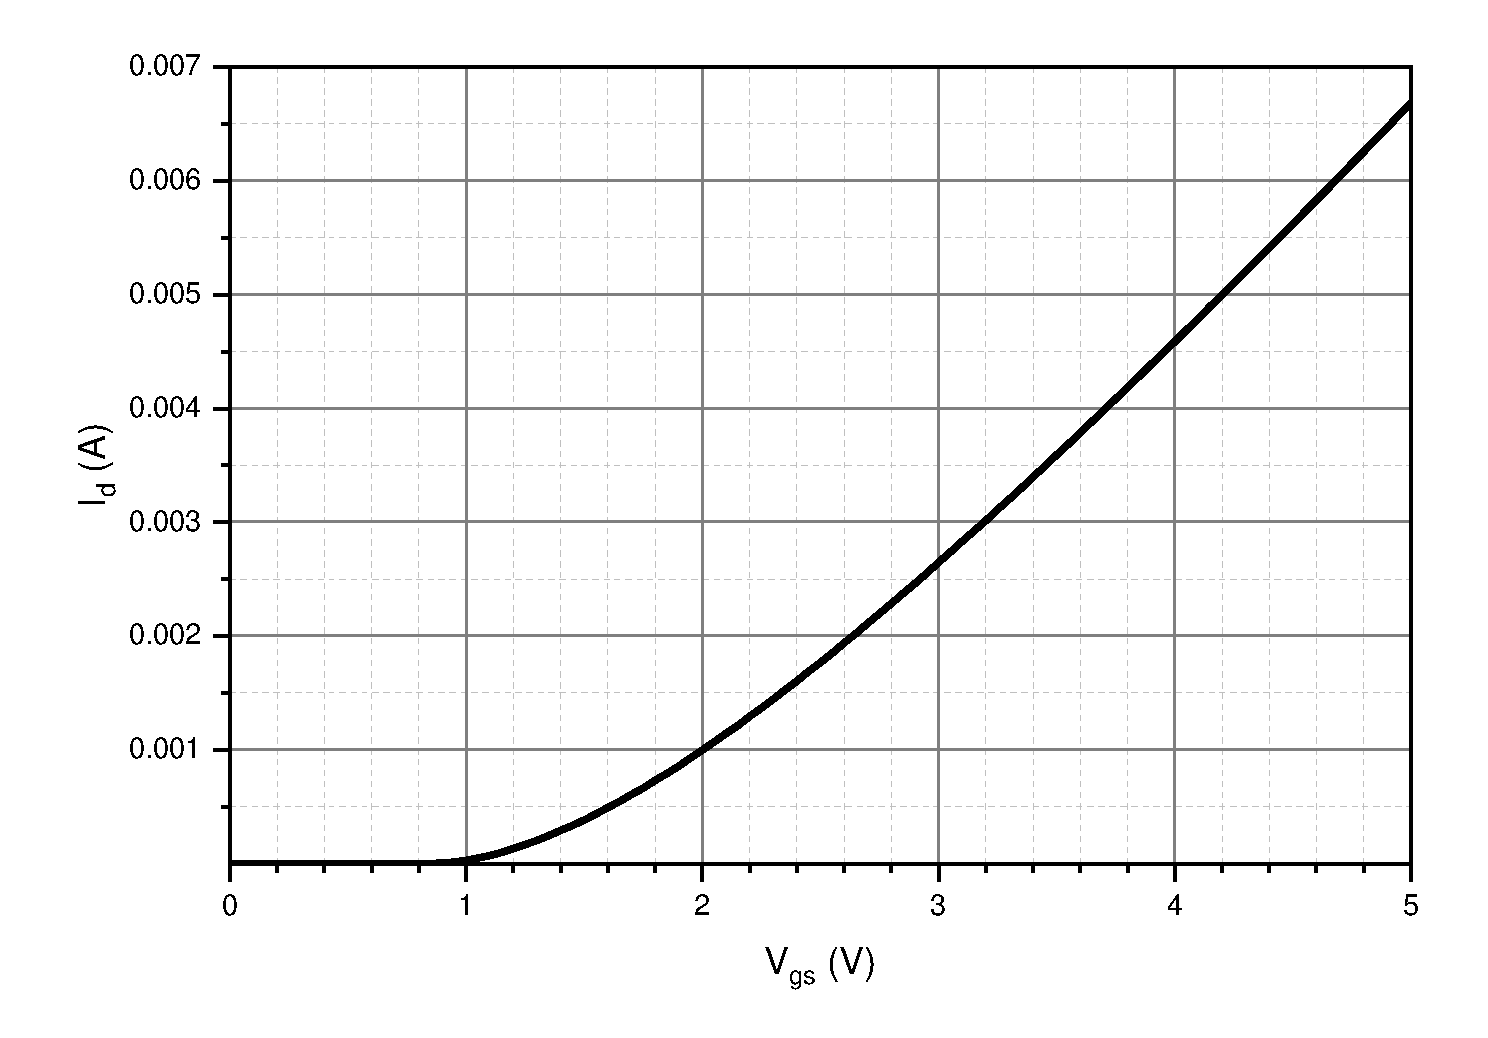
\includegraphics[width=\linewidth]{Figures/E1_NMOS_Characteristic/Id_vgs_linear}
			\caption{}
			\label{fig:idVgsLinear}
		\end{subfigure}
		\begin{subfigure}{0.48\linewidth}
			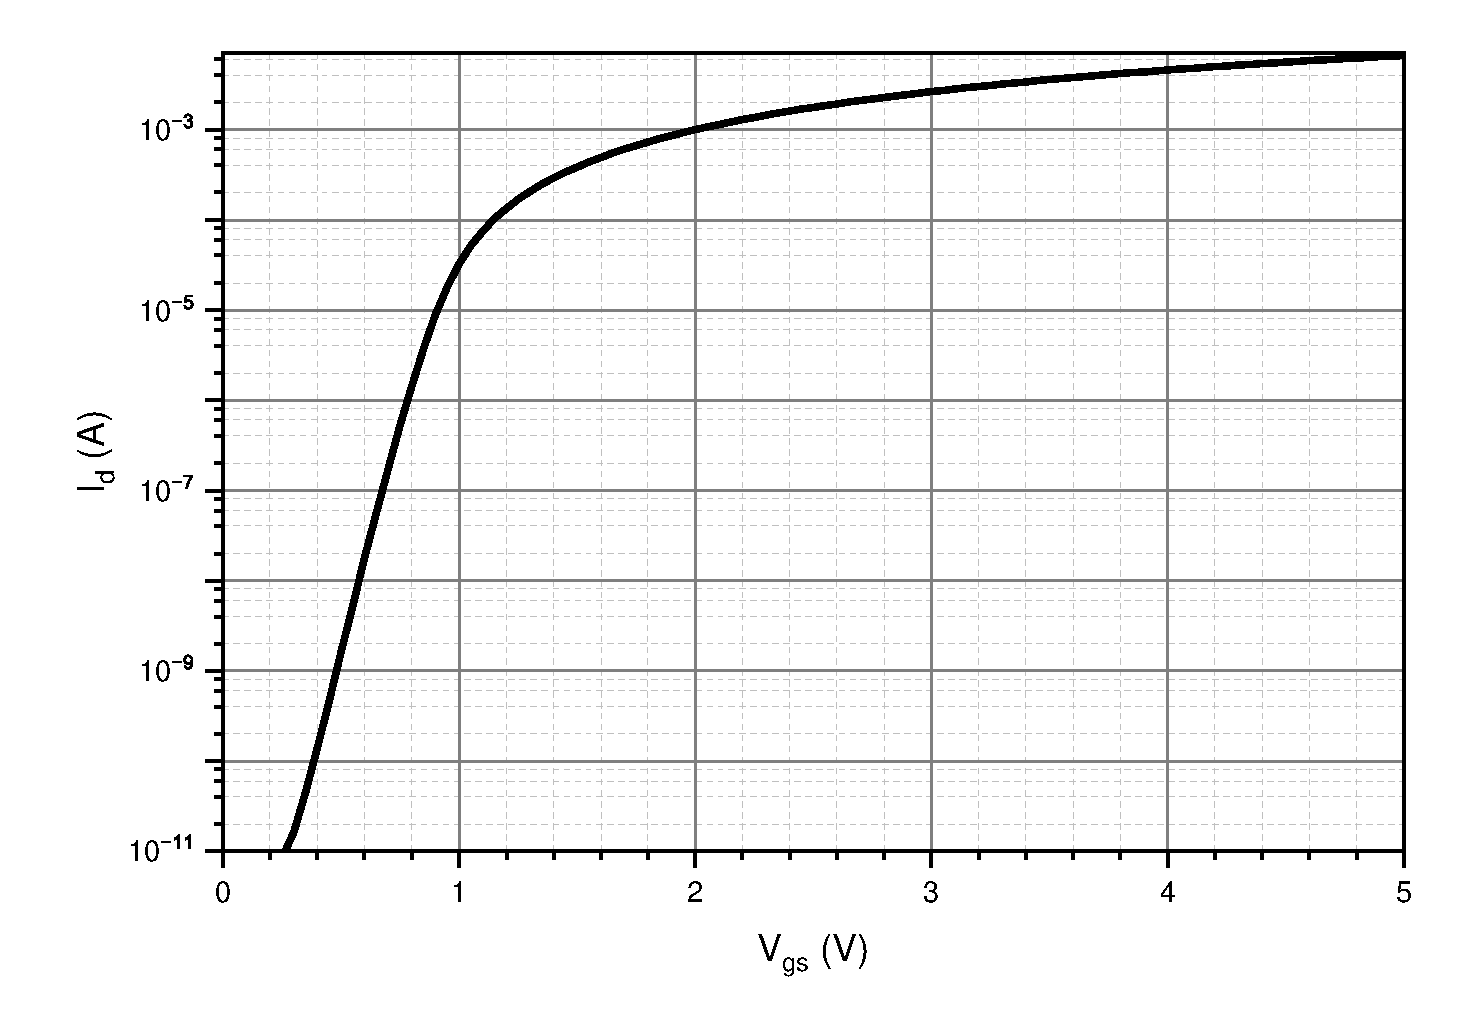
\includegraphics[width=\linewidth]{Figures/E1_NMOS_Characteristic/Id_vgs_log}
			\caption{}
			\label{fig:idVgsLog}
		\end{subfigure}
		\caption{Plot of $I_{D}$ against $V_{GS}$ in (a) linear scale and (b) log scale when $V_{DS} = \SI{5}{\volt}$}
	\end{figure}
	
	The sub-threshold slope is defined as:
	\begin{equation}
		S = \frac{\partial V_{GS}}{\partial \left(\log I_D\right)} \approx \frac{\Delta V_{GS}}{\Delta \left(\log I_D\right)}
	\end{equation}
	To get the slope, I choose to substitute in the value of $\log(I_D)$ when $V_{GS} = \SI{0.4}{\volt}$ and $\SI{0.8}{V}$:
	\begin{equation}
		S \approx \frac{0.8 - 0.4}{-5.835 - \left(-9.852\right)} = 99.6 \times 10^{-3}\ \si{\volt\per\decade}
	\end{equation}
	
	When $V_{GS} = \SI{0}{\volt}$, there's a finite size of current, which is measured to be around $\SI{5.01}{\pico\ampere}$. This current is caused due to the internal structure of the MOSFET. When switched off, the diodes are formed between bulk and drain and bulk and source as shown in Figure~\ref{fig:bodyDiode}. As source and bulk are connected together in this case, the diode between source and bulk is shorted, and only left with the diode between drain and bulk or equivalently drain and source. When there's voltage applied between drain and source, the diode will be reverse biased and there will be a small reverse saturation current. The measured $\SI{5.01}{\pico \ampere}$ is probably caused by this.
	
	\begin{figure}[htbp]
		\centering
		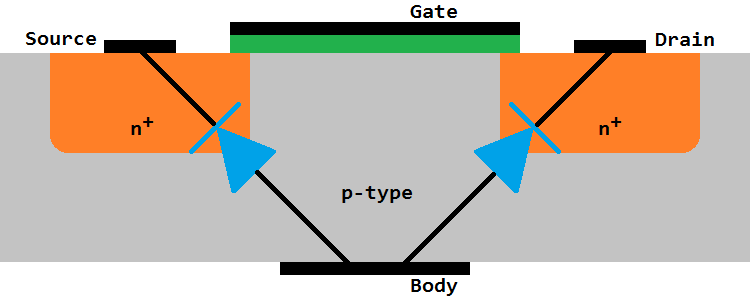
\includegraphics[width = 0.5\linewidth]{Figures/E1_NMOS_Characteristic/Body_diode}
		\caption{The diode formed between drain and bulk and source and bulk}
		\label{fig:bodyDiode}
	\end{figure}
	
	\newpage
	
	\section{Exercise 2: Common-Source Amplifier}
	
	The circuit shown in Figure~\ref{fig:invAmp} is called the inverting amplifier or common-source amplifier, Figure~\ref{fig:dcResponse} shows it's large signal DC input output characteristic. In saturation region of this amplifier, the output voltage changes largely for even a small change in input voltage, and thus it could be used for amplifying signal.
	\begin{figure}[htbp]
		\centering
		\begin{subfigure}[c]{0.48\linewidth}
			\centering
			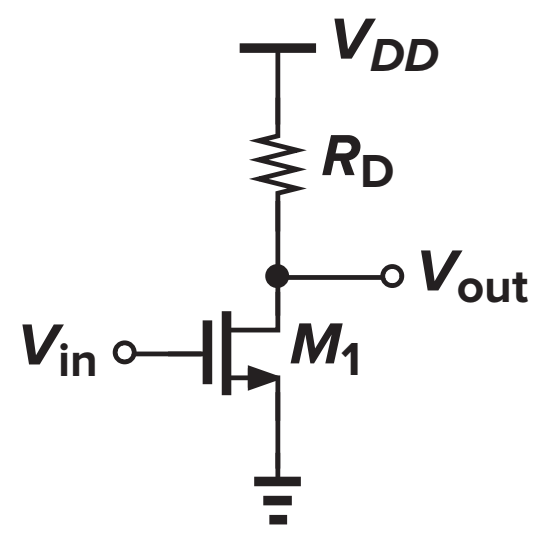
\includegraphics[width=0.5\linewidth]{Figures/E2_Inverting_Amplifier/Inv_amp}
			\caption{}
			\label{fig:invAmp}
		\end{subfigure}
		\begin{subfigure}[c]{0.48\linewidth}
			\centering
			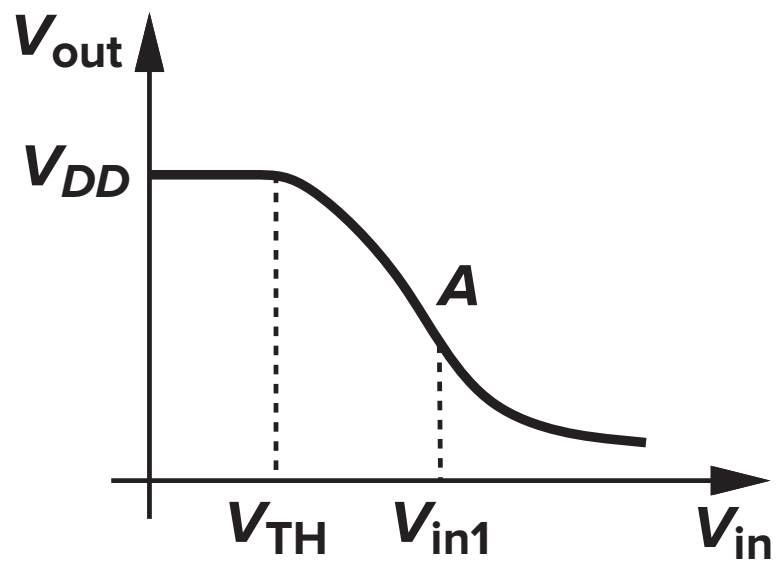
\includegraphics[width=0.7\linewidth]{Figures/E2_Inverting_Amplifier/DC_response}
			\caption{}
			\label{fig:dcResponse}
		\end{subfigure}
		\caption{(a) The circuit of common-source amplifier (b) The large signal DC response of amplifier}
	\end{figure}
	
	The small signal gain of this amplifier is given as:
	\begin{equation}
		A_v = \frac{V_{out}}{V_{in}} = -g_m \left(R_D \parallel r_o\right)
		\label{eq:invAmpGain}
	\end{equation}
	In which $R_{D}$ is the resistor connected between $V_{DD}$ and drain of NMOS, and $r_o$ is the output resistance calculated in equation \eqref{eq:outputResistance}. Taking $R_D = \SI{100}{\kilo\Omega}$, the DC simulation shows the input operating point to be $V_{in,DC} = \SI{0.983}{\volt}$ and the amplitude to be $\SI{0.1}{\milli\volt}$ to make sure the maximum dynamic range and linearity. The transient simulation at $\SI{1}{\kilo\hertz}$ is shown in Figure~\ref{fig:tran1k}.
	
	\begin{figure}[htbp]
		\centering
		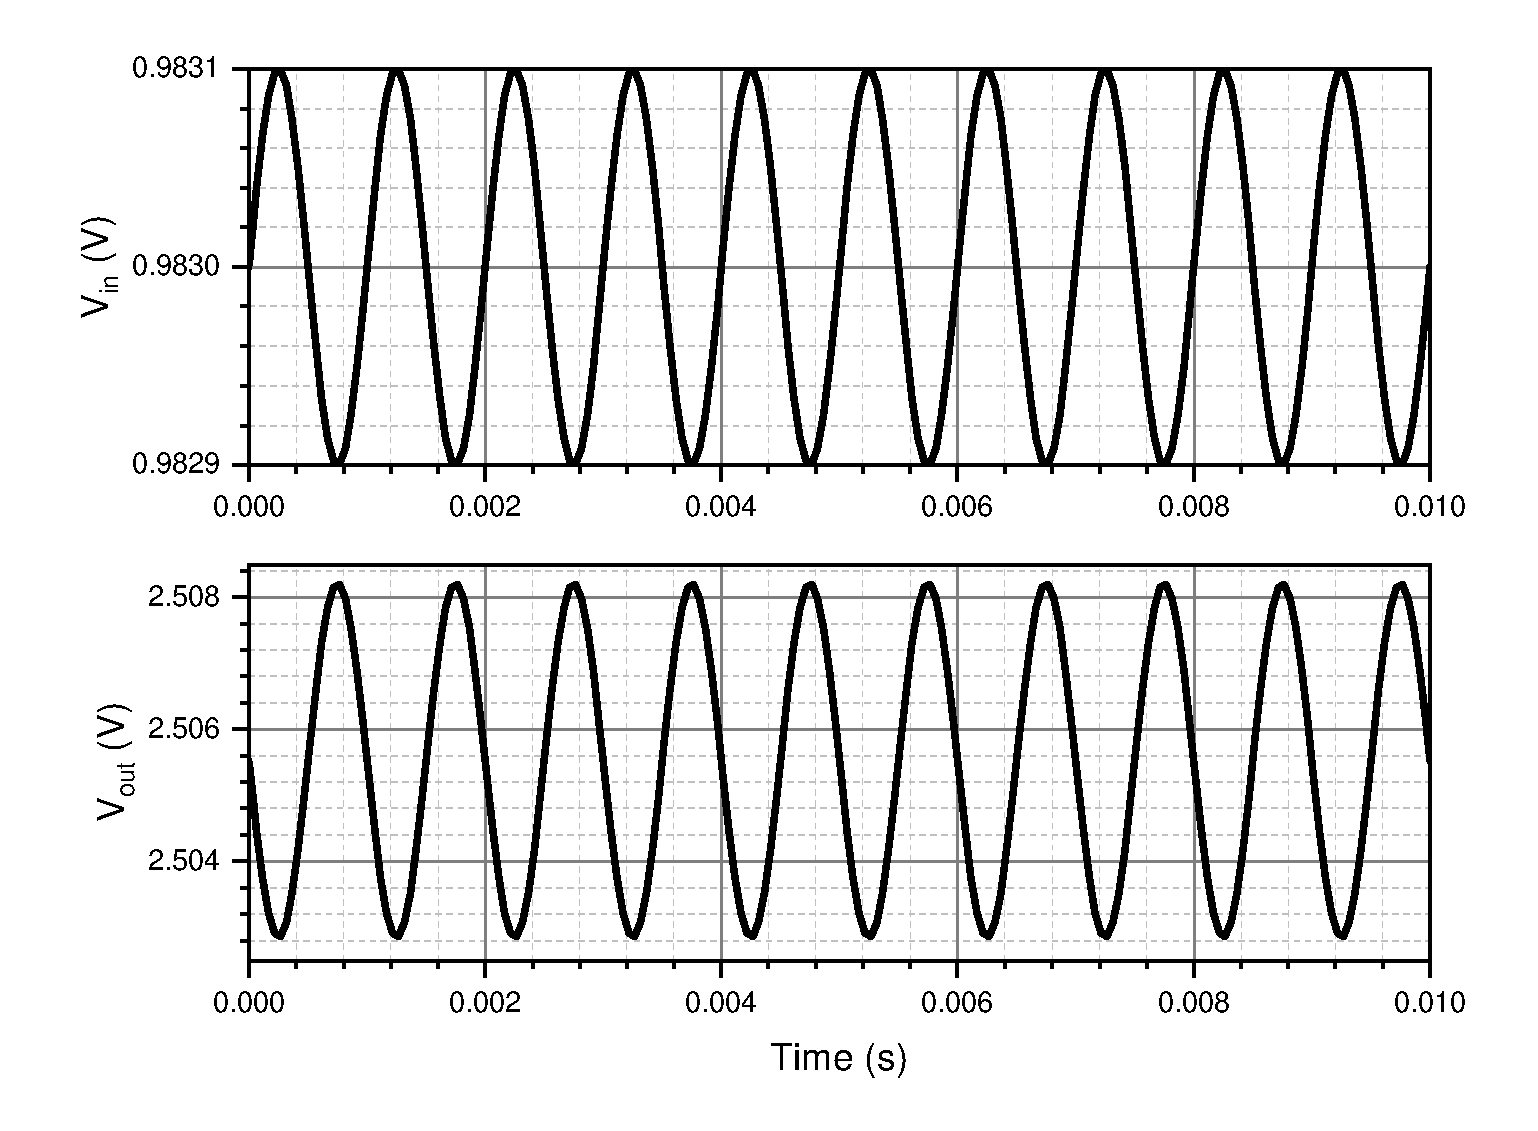
\includegraphics[width=0.7\linewidth]{Figures/E2_Inverting_Amplifier/Vin_Vout_1k}
		\caption{Transient simulation of amplifier with input signal at frequency of \SI{1}{\kilo\hertz}}
		\label{fig:tran1k}
	\end{figure}
	
	The gain of the amplifier is measured via the quotient of peak to peak of input and peak to peak of output. The peak to peak input is twice of amplitude, which is $\SI{0.2}{\milli\volt}$. The output peak to peak value is measured to be $\SI{5.33}{\milli\volt}$. This gives the overall transient gain:
	\begin{equation}
		A_v = \frac{V_{out,\ \text{peak to peak}}}{V_{in,\ \text{peak to peak}}} = \frac{5.33}{0.2} = -26.65
		\label{eq:transGain}
	\end{equation}
	As mentioned in equation~\eqref{eq:invAmpGain}, the gain is directly proportional to the parallel resistance of output resistance $r_o$ and the resistance of the resistor $R_D$. If $R_D$ keep increases, the parallel resistance will be smaller, and thus reduce the gain.
	
	The frequency response of the amplifier could be measured using the AC simulation, a Bode diagram that measures the frequency response of the circuit between $\SI{1}{\hertz}$ and $\SI{1}{\giga\hertz}$ is shown in Figure~\ref{fig:ac_analysis_inv}. The low frequency gain of this amplifier is measured to be $-26.80$, which matches the result calculated in transient analysis (equation~\eqref{eq:transGain}). The gain starts to drop at high frequency, the $\SI{-3}{\decibel}$ bandwidth of the amplifier is measured to be around $\SI{65}{\mega\hertz}$.
	
	\begin{figure}[htbp]
		\centering
		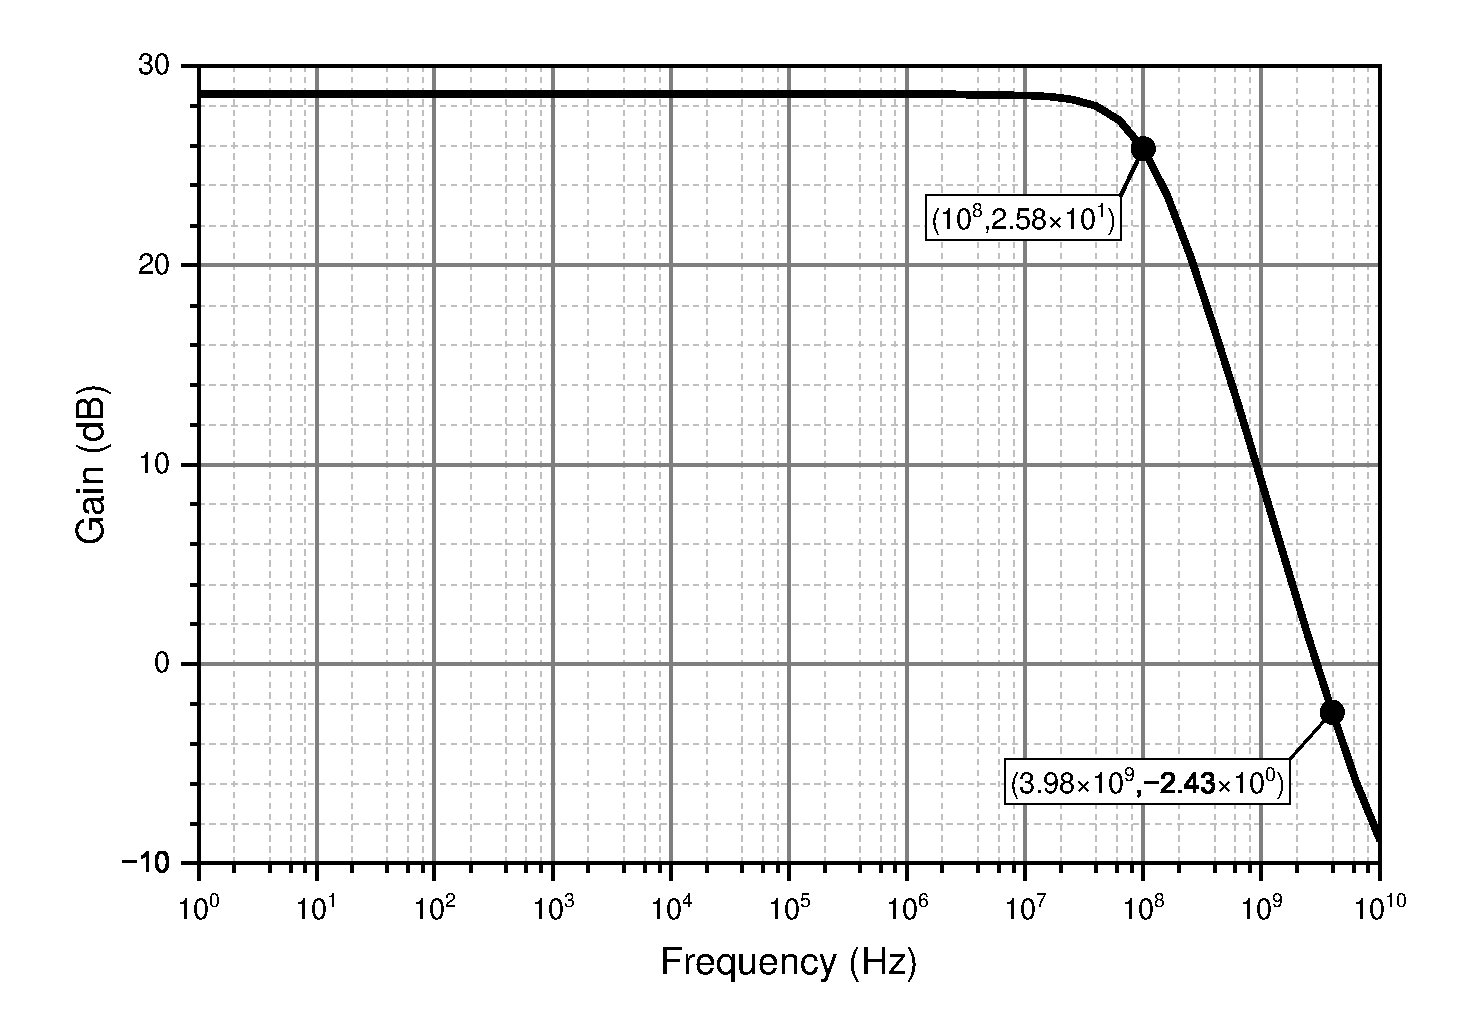
\includegraphics[width=0.7\linewidth]{Figures/E2_Inverting_Amplifier/AC_analysis}
		\caption{Transient simulation of amplifier with input signal at frequency of \SI{1}{\kilo\hertz}}
		\label{fig:ac_analysis_inv}
	\end{figure}
	
	Another transient simulation is taken to measure the gain of the amplifier at $\SI{100}{\mega\hertz}$, which is outside the bandwidth of the amplifier, this gives the gain to be $19.05$, which is different from the measured value $14.23$ in AC simulation.
	
	If the circuit is built in reality, the actual frequency response of the circuit would possibly be way worse than the measured result. This is because in reality, there's more capacitance between pins and wires while the model here only considers the parasitic capacitance in the MOSFET.
	
	\newpage
	
	\section{Exercise 3: Current Mirror}
	
	The circuit of the current mirror is shown in Figure~\ref{fig:currentMirror}, ideally the current flowing through the two MOSFET should be exactly the same as their gate voltage is the same and in saturation region the voltage is almost constant. In the simulation, the drain terminal of MOSFET $M_2$ is connected to $V_{DD}$ and $I_{REF}$ is set to $\SI{100}{\micro\ampere}$. The measured output current is $\SI{109.64}{\micro\ampere}$ which shows a slight offset.
	
	\begin{figure}[htbp]
		\centering
		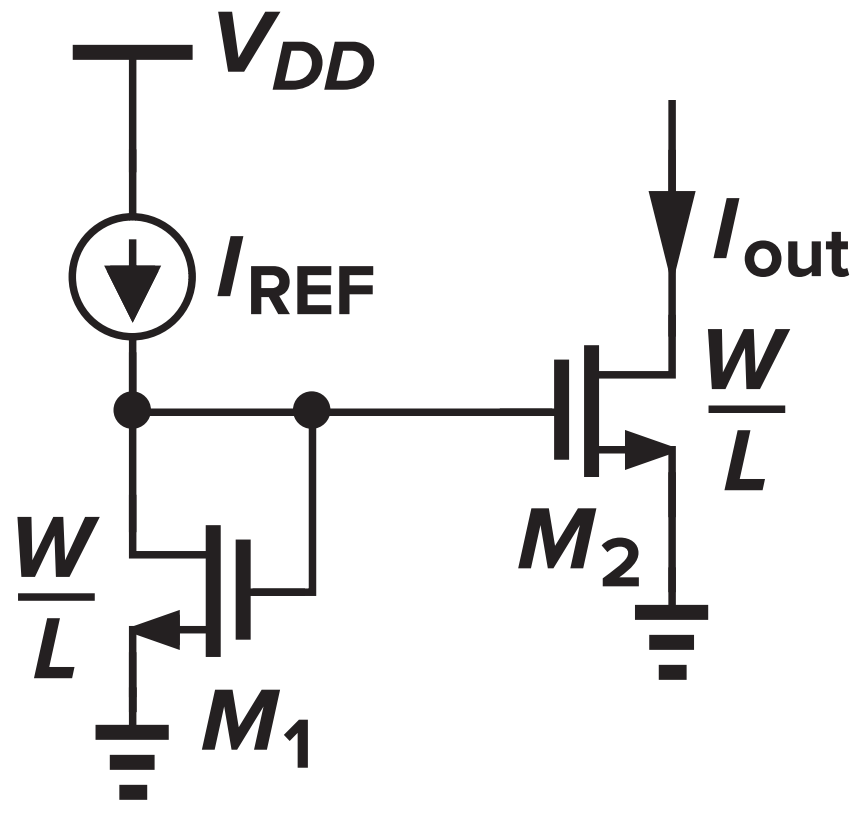
\includegraphics[width=0.35\linewidth]{Figures/E3_Current_Mirror/current_mirror}
		\caption{Basic current mirror circuit}
		\label{fig:currentMirror}
	\end{figure}
	
	Figure~\ref{fig:ioutIin} shows the plot of $I_{out}$ against $I_{in}$ when the MOSFET $M_2$ has it's drain connected to $V_{DD}$, and Figure~\ref{fig:ioutVgs} shows the plot of $I_{out}$ against $V_{DS}$ under a constant value of $I_{in} = \SI{100}{\micro\ampere}$.
	
	\begin{figure}[htbp]
		\centering
		\begin{subfigure}{0.48\linewidth}
			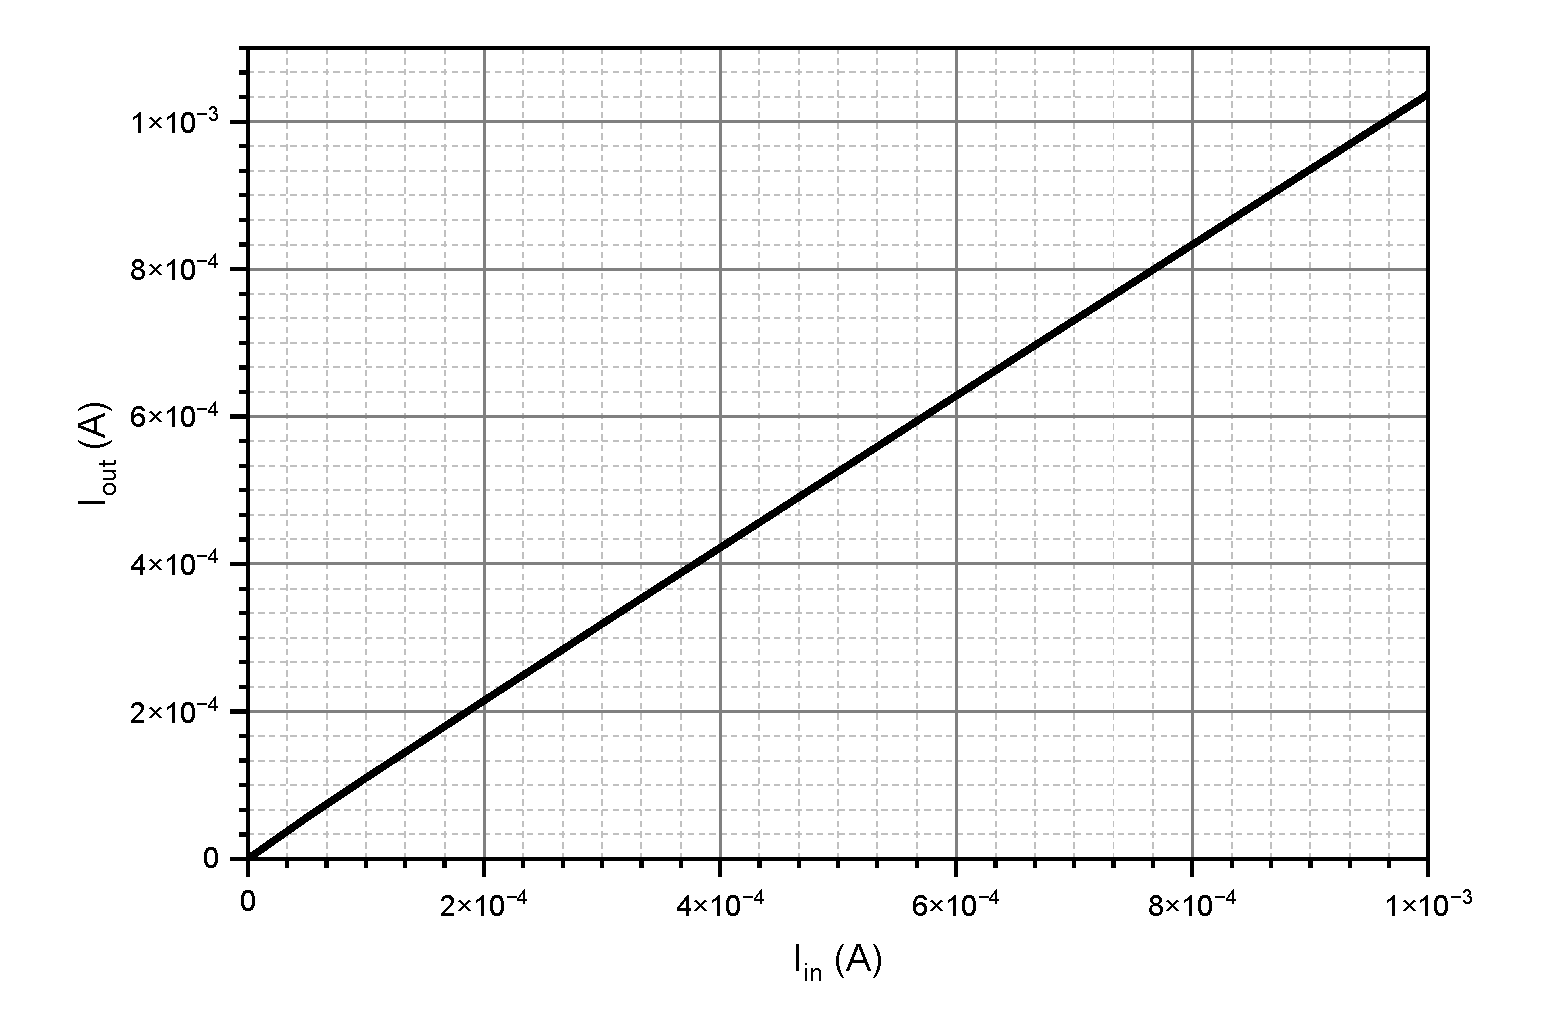
\includegraphics[width=\linewidth]{Figures/E3_Current_Mirror/Iin_Iout}
			\caption{}
			\label{fig:ioutIin}
		\end{subfigure}
		\begin{subfigure}{0.48\linewidth}
			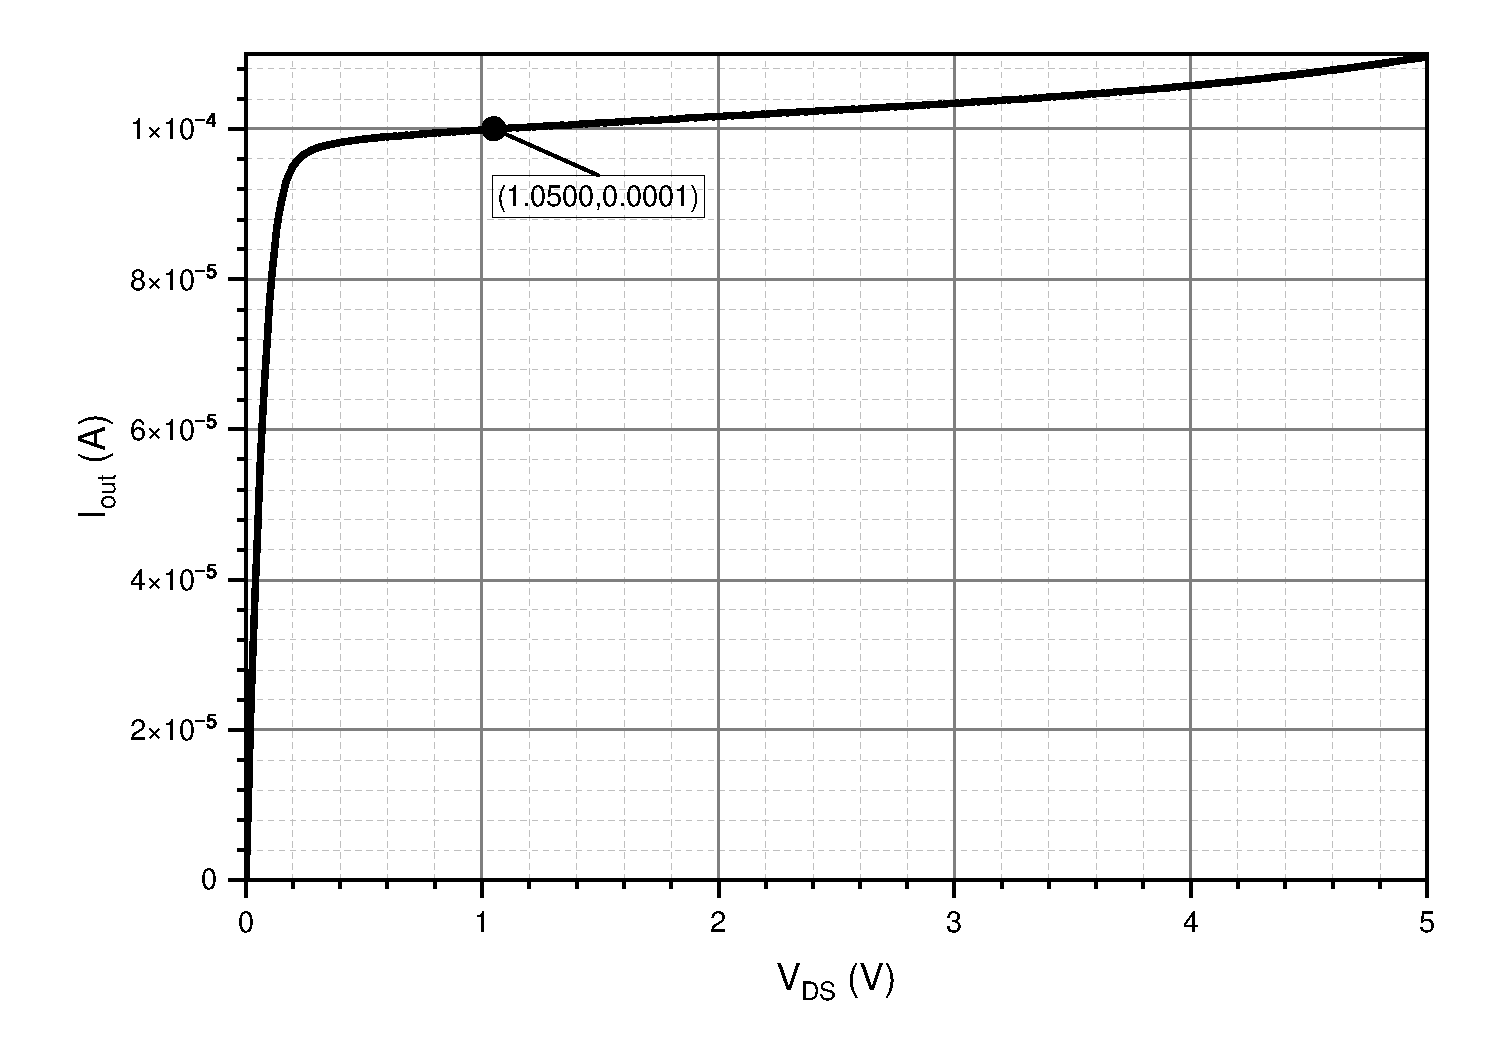
\includegraphics[width=\linewidth]{Figures/E3_Current_Mirror/Iout_Vds}
			\caption{}
			\label{fig:ioutVgs}
		\end{subfigure}
		\caption{Plot of (a) output current against input current and (b) output current against $V_{DS}$}
	\end{figure}
	
\end{document}
